%!TEX root=./paper.tex
\subsection{\textbf{Model input}}

For each node, we create a feature vector that represents all the information related to that node. The feature vector for a node is composed of three feature vectors that are, as defined ahead, concatenated:

\subsubsection{Graph embedding generation using Node2Vec:}

In order for the model to effectively learn the spatial relationships between the detector nodes based on graph structure, we need a way to generate an appropriate representation of the graph nodes that capture the neighborhood structure effectively. $Node2Vec$\cite{node2vec} is a feature learning algorithm that uses second-order biased random walks in a Skip-gram architecture to learn feature vectors for nodes in the graph. There are two key steps for feature generation:

\begin{enumerate}[(i)]
    \item \textit{Sampling using second-order biased random walks}: Two hyper-parameters \( p \) and \( q \) are introduced, which are the "return" and "in-out" parameters, respectively. Suppose we simulate a random walk of fixed length \( l \). Let \( c_i \) denote the \( i \)th node in the walk, starting with \( c_0 = u \). Nodes \( c_i \) are generated by the following distribution:
    \[
        P(c_i = x \mid c_{i-1} = v) =
        \begin{cases}
        \frac{\pi_{vx}}{Z} & \text{if } (v,x) \in E \\
        0 & \text{otherwise}
        \end{cases}
    \]
    where \( \pi_{vx} \) is the unnormalized transition probability between nodes \( v \) and \( x \), and \( Z \) is the normalizing constant.
    
    For a walk that just traversed edge \( (t,v) \) and now resides at node \( v \), we now need to decide on the next step so it evaluates the transition probabilities \( \pi_{vx} \) on edges \( (v,x) \) leading from \( v \). The transition probability \( \pi_{vx} = \alpha_{pq}(t,x)\cdot w_{vx} \), where 
    \[
        \alpha_{pq}(t,x) = 
        \begin{cases}
        \frac{1}{p}  & \text{if } d_{tx} = 0\\
        1 & \text{if } d_{tx} = 1\\
        \frac{1}{q} & \text{if } d_{tx} = 2
        \end{cases}
    \]
    and \( d_{tx} \) denotes the shortest path distance between nodes \( t \) and \( x \).

    \item \textit{Optimizing objective function using Skip-gram}: Let for graph \( G(V, E) \), \( f: V \rightarrow \mathbb{R}^d \) be the \( d \)-dimensional feature representation function. Thus, \( f \) is a matrix of size \( |V| \times d \) parameters. Now, for every node \( u \in V \), we define \( N_S(u) \subset V \) as a \emph{network neighborhood} of the node \( u \) generated in step (i). Define similarity between two nodes \( u \) and \( v \) as:
    \[
        P_f(v|u) = \frac{\exp(f(v)^T f(u))}{\sum_{w \in V} \exp(f(w)^T f(u))} \tag{1}
    \]
    For neighborhood \( N_s(v) \) of \( v \), define the probability of the neighborhood of \( u \) as:
    
    \[ P_f(N_s(u)|u) = \prod_{v \in N_s(u)} P_f(v|u) \tag{2} \]

    Further, the global neighborhood likelihood for a given \( f \) can be define as:
    \[ \sum_{u \in V} \log P_f(N_s(u)|u) \tag{3}\]
    which is the objective function that we want to maximize through the feature representation function \(f\). Hence,
     \[
    \max_{u \in V} \sum_{u \in V} \log \left( \prod_{v \in N_s(u)} \frac{\exp(f(v)^T f(u))}{\sum_{w \in V} \exp(f(w)^T f(u))} \right) \tag{4}
    \]
\end{enumerate}

\begin{figure*}[htbp]
  \centering
  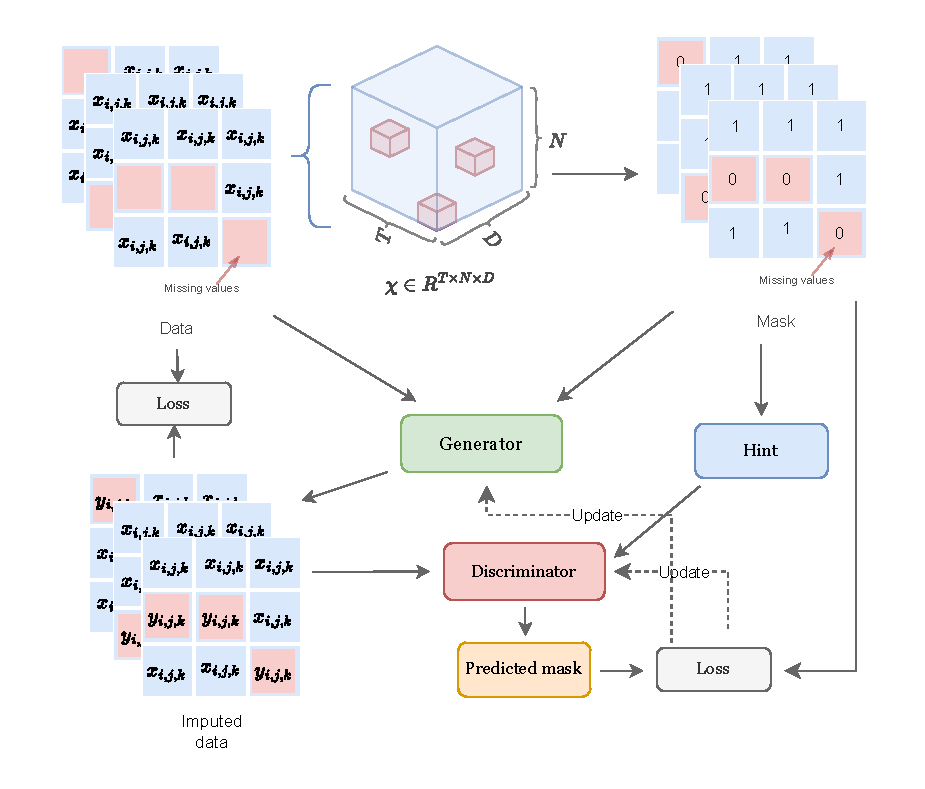
\includegraphics[width=0.85\textwidth]{model.pdf}
  \caption{Model architecture}
  \label{fig:dataset}
\end{figure*}

\subsubsection{Traffic volume normalised:}
The input data should be normalized to increase the training speed and effectiveness. The traffic volume counts at different detectors are normalized as follows:
\[
x_{\text{norm}} = \frac{x - x_{\text{min}}}{x_{\text{max}} - x_{\text{min}}}
\]
Thus, \( x_{\text{norm}} \) is in the range \([0,1]\) after normalization. This same approach is used for other continuous or discrete single-valued features.

\subsubsection{Word2Vec encoding of other exogenous variables:}
Skip-gram\cite{skipgram}, a popular Word2Vec\cite{word2vec} architecture, aims to predict the context words given a target word. It learns to encode the semantic meaning of words by maximizing the probability of context words given the target word. Mathematically, the objective function for Skip-gram can be represented as:

\[
J_\theta = \frac{1}{T}\sum^{T}_{t=1}\sum_{-n\leq j \leq n, j \neq 0}\log p\left(w_{j+1} \mid w_{t}\right)
\]

where \( w_t \) represents the target word at position \( t \), \( c \) is the size of the context window, and \( T \) is the total number of words in the corpus.

We use \textit{Word2Vec} to encode the other possibly relevant exogenous variables, like weather, road type, etc., as features to the model input, thus increasing its effectiveness. We would like to note that this approach is easily extensible to any number of other features that may prove to be relevant in the future, and we wish to add to the model input.

\vspace{3ex} Concatenating the feature vectors from the above sub-parts, we get the final input vector. Extending the notation as defined in section III.A, for \(N\) nodes, we define the construction of \(\mathbf{x}_i^t\), the feature vector of the node \(i\) at time \(t\). Assuming \textit{Node2Vec} was used as defined in (i) to generate \(R^{D_g}\) dimensional graph embeddings for each node. Let \(g_i\) be the graph embedding for node \(i\). Then, for \(n\) single-dimensional real-valued features \((r_1, r_2, \ldots, r_n)\), let them be normalized as defined in (ii) to \((r_1^{\text{norm}}, r_2^{\text{norm}}, \ldots, r_n^{\text{norm}})\) thus creating a \(D_n = n\) dimensional vector. Let them be represented by \(h_i^t\). Finally, for \(m\) "words" representing other semantic information related to the node, and using \textit{Word2Vec} to output \(d_w\) dimensional vectors for each word, we get a \(R^{mxd_w}\) dimensioned vector that we flatten and represent as \(k_i^t\) \(\in\) \(R^{D_w}\) where \(D_w = m \times d_w\).

Finally, one concatenation of the above three, we get the feature vector of node \(i\) at time \(t\) 
\[\mathbf{x}_i^t = (\ g_i\ ||\ h_i^t\ ||\ k_i^t\ ) \in R^D\] 
where \(D = D_g+D_n+D_w\).
Thus, from (i) and (ii), over \( T \) consecutive time steps and for \( N \) nodes, we get the final feature vector as \( \mathbf{\chi} \)  \(\in\) \( \mathbb{R}^{T \times N \times D} \).
Depending on the task, we also add other task-specific inputs like for the case of imputation a binary matrix \( M \) representing the missing and known values. Specific implementation details are discussed further in the experiments section.